\documentclass{beamer}
\usepackage{graphicx}

\usetheme{Singapore}
\usecolortheme{crane}

\title{Določanje $\pi$ z metodo Monte Carlo} 
\author[Matic Plut]{Matic Plut \\ 23211109}
\date{\today}
\logo{
    
\includegraphics[width=3cm]{logo_FS.jpg}
    }

\begin{document}

\begin{frame}
    \titlepage
\end{frame}
\logo{}

\section{Metoda Monte Carlo}

\begin{frame}
    \frametitle{Kazalo}
    \tableofcontents[currentsection]
\end{frame}

\begin{frame}{Metoda Monte Carlo}
    Z metodo Monte Carlo $\pi$ izračnunamo iz razmerja ploščin kvadrata s stranico $a = 2r = 2$ in kroga $r = 1$.
    \\
    Ploščine aproksimiramo tako da v območju kvradata generiramo veliko št. naključnih točk.

    \begin{figure}
      \centering
      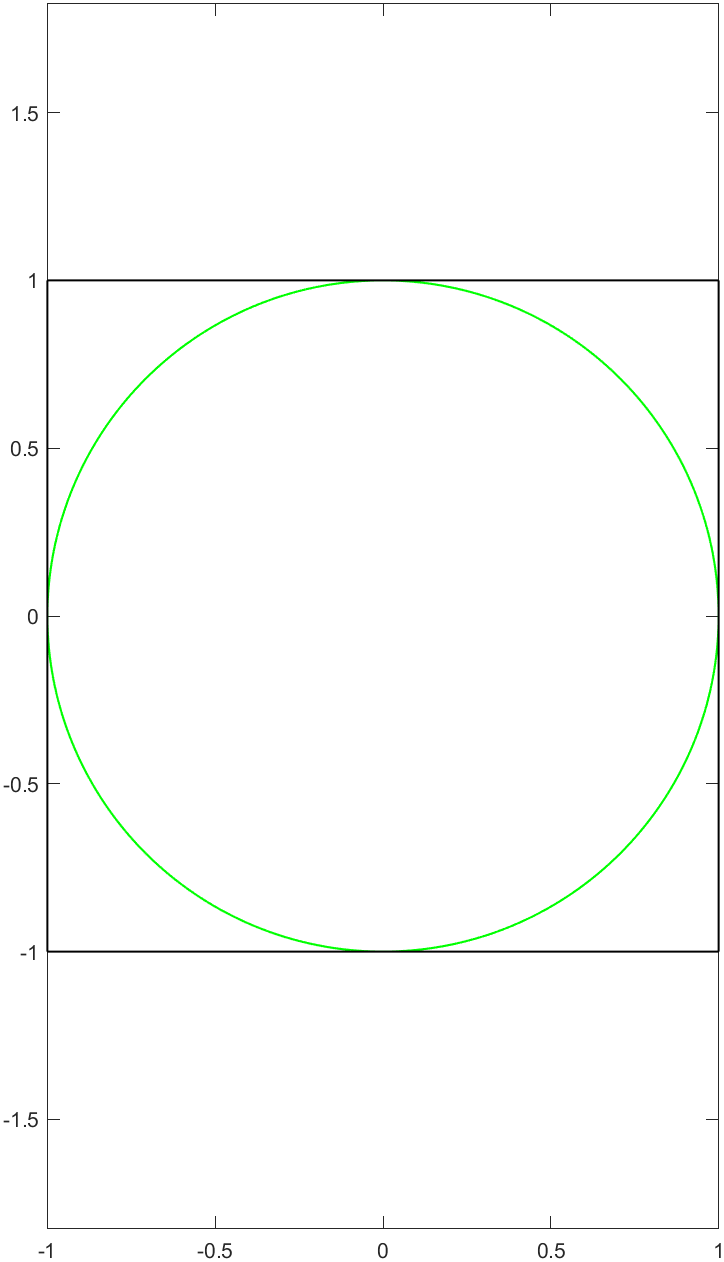
\includegraphics[height=6cm]{graf.png}
    \end{figure}
\end{frame}

\begin{frame}{Formula za izračun}
    Formulo za izračun $\pi$ izpeljemo iz ploščin obeh likov.\\
    $$A_{kv}=a^2,~A_{kr}=\pi r^2;~a=2r,~r=1$$\\
    $$\pi = 4\frac{A_{kr}}{A_{kv}}=4\frac{št.~točk~v~krogu}{št.~vseh~točk}$$
\end{frame}

\section{Implementacija v MatLab}

\begin{frame}
    \frametitle{Kazalo}
    \tableofcontents[currentsection]
\end{frame}

\begin{frame}{Generiranje in preverba točk}

    Točke generiramo tako, da z funkcijo rand(), ki generira matriko z elementi med 0 in 1.\\
    posebaj generiramo x in y koordinate in jih transformiramo na naše območje.
    
    \begin{figure}
          \centering
          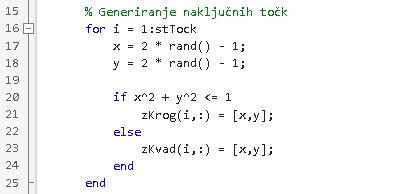
\includegraphics[height=4cm]{generiranje_točk.JPG}
    \end{figure}

\end{frame}

\begin{frame}{Izračun $\pi$ in napake}
    Iz razvrščenih točk nato po formuli izračunamo približek $\pi$ in odstopanje od prave vredsoti.
    
    \begin{figure}
          \centering
          
\includegraphics[width=12cm]{izračun.JPG}
    \end{figure}

\end{frame}

\section{Rezultati}

\begin{frame}
    \frametitle{Kazalo}
    \tableofcontents[currentsection]
\end{frame}

\begin{frame}{}
    
    \begin{figure}
          \centering
          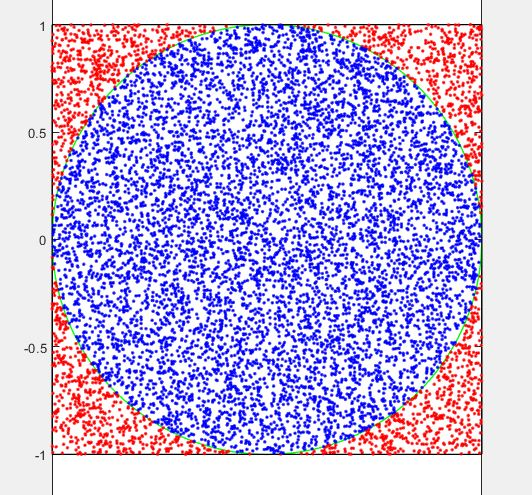
\includegraphics[height=7cm]{Točke.JPG}
          \caption{Prikaz naključno generiranih točk.}
    \end{figure}

\end{frame}

\begin{frame}

    \begin{figure}[Prikaz naključno generiranih točk]
          \centering
          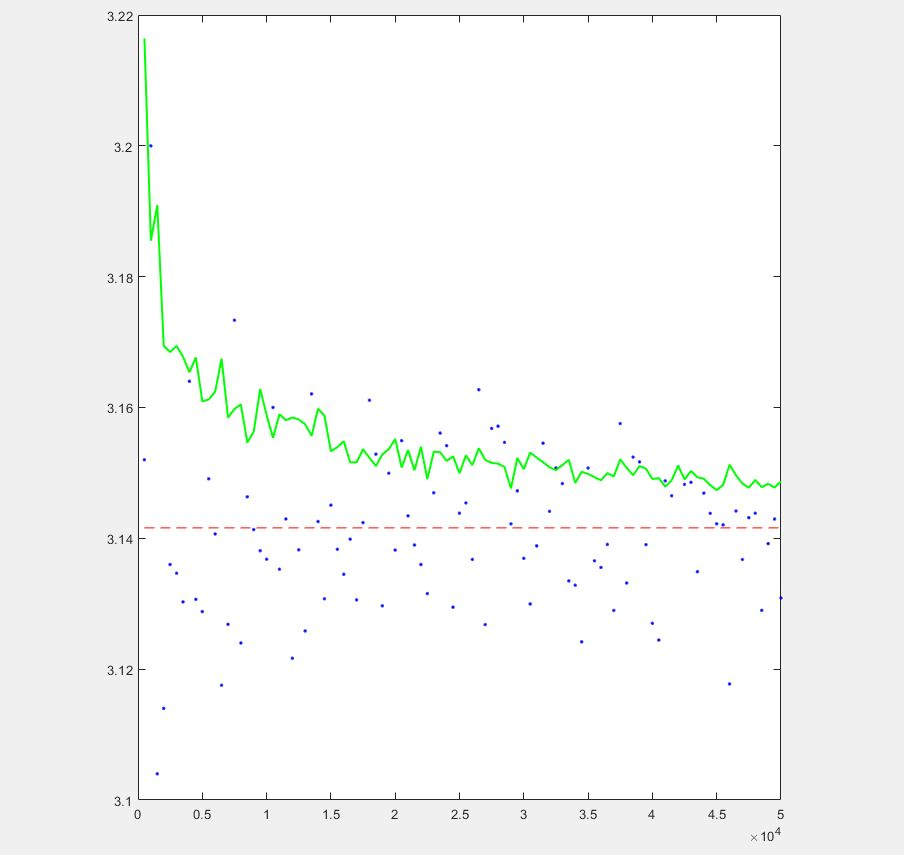
\includegraphics[height=7cm]{odstopanje.JPG}
          \caption{Prikaz povprečnega odstopanje metode od prave vrednosti $\pi$.}
    \end{figure}

\end{frame}

\end{document}